\chapter{Databasen}
Nedenfor følger design af software til databasen og dens interface. Dette er lavet på baggrund af kravspecifikation og systemarkitektur. 


\subsection{Modulets Ansvar}
Databasen er der hvor havneterminalens personale kan aflæse data fra skibet. Disse data er sendt fra KI. Programmerne indeholder brugergrænseflader, der opfylder kravene beskrevet i kravspecifikationen. Her kan der også ses en prototype på brugergrænsefladen.
Databasemodulet har tre dele; serveren, websiden og en MySQL-database. \\
\textbf{Serveren} står for kommunikationen immellem KI og Databasen. Serveren modtager data fra KI og lagrer disse i en tekstfil.\\
\textbf{Webinterfacet} giver brugeren mulighed for at se info om BROS samt at logge sig ind i BROS-databasen hvorfrax data om skibe, der er tilsluttet systemet, kan aflæses. Webinterfacets tre vigtigste funktioner er at gemme ny data til MySQL-databasen, slette den tekstfil som serveren lavede og vise data for brugeren. For at håndtere webinterfacet, der benytter sig af php (webprogrammering) kræves der en webserver, som er i stand til at håndtere dette. En af de mest udbredte er apacheserveren, som også benyttes for denne webside.
\textbf{MySQL-databasen} er en database, som er  installeret på computeren. Alle data, som er sendt fra KI, er lagret i MySQL-databasen.

\subsection{State machine diagram}
Designet af Databasen tager udgangspunkt i arkitekturen fremstillet i artefaktet Systemarkitektur. Her blev der fremstillet et state machine for serveren webinterfacet. State machinet var simplificeret og er i designfasen blevet udvidet. Resultatet ses i \textit{figur \ref{fig:stm_server}} for serveren og \textit{figur \ref{fig:stm_web}} webinterfacet. Figuren beskriver hvilke stadier programmet kan befinde sig i og sammenhængen imellem dem.

\begin{figure}[H]
	\centering
	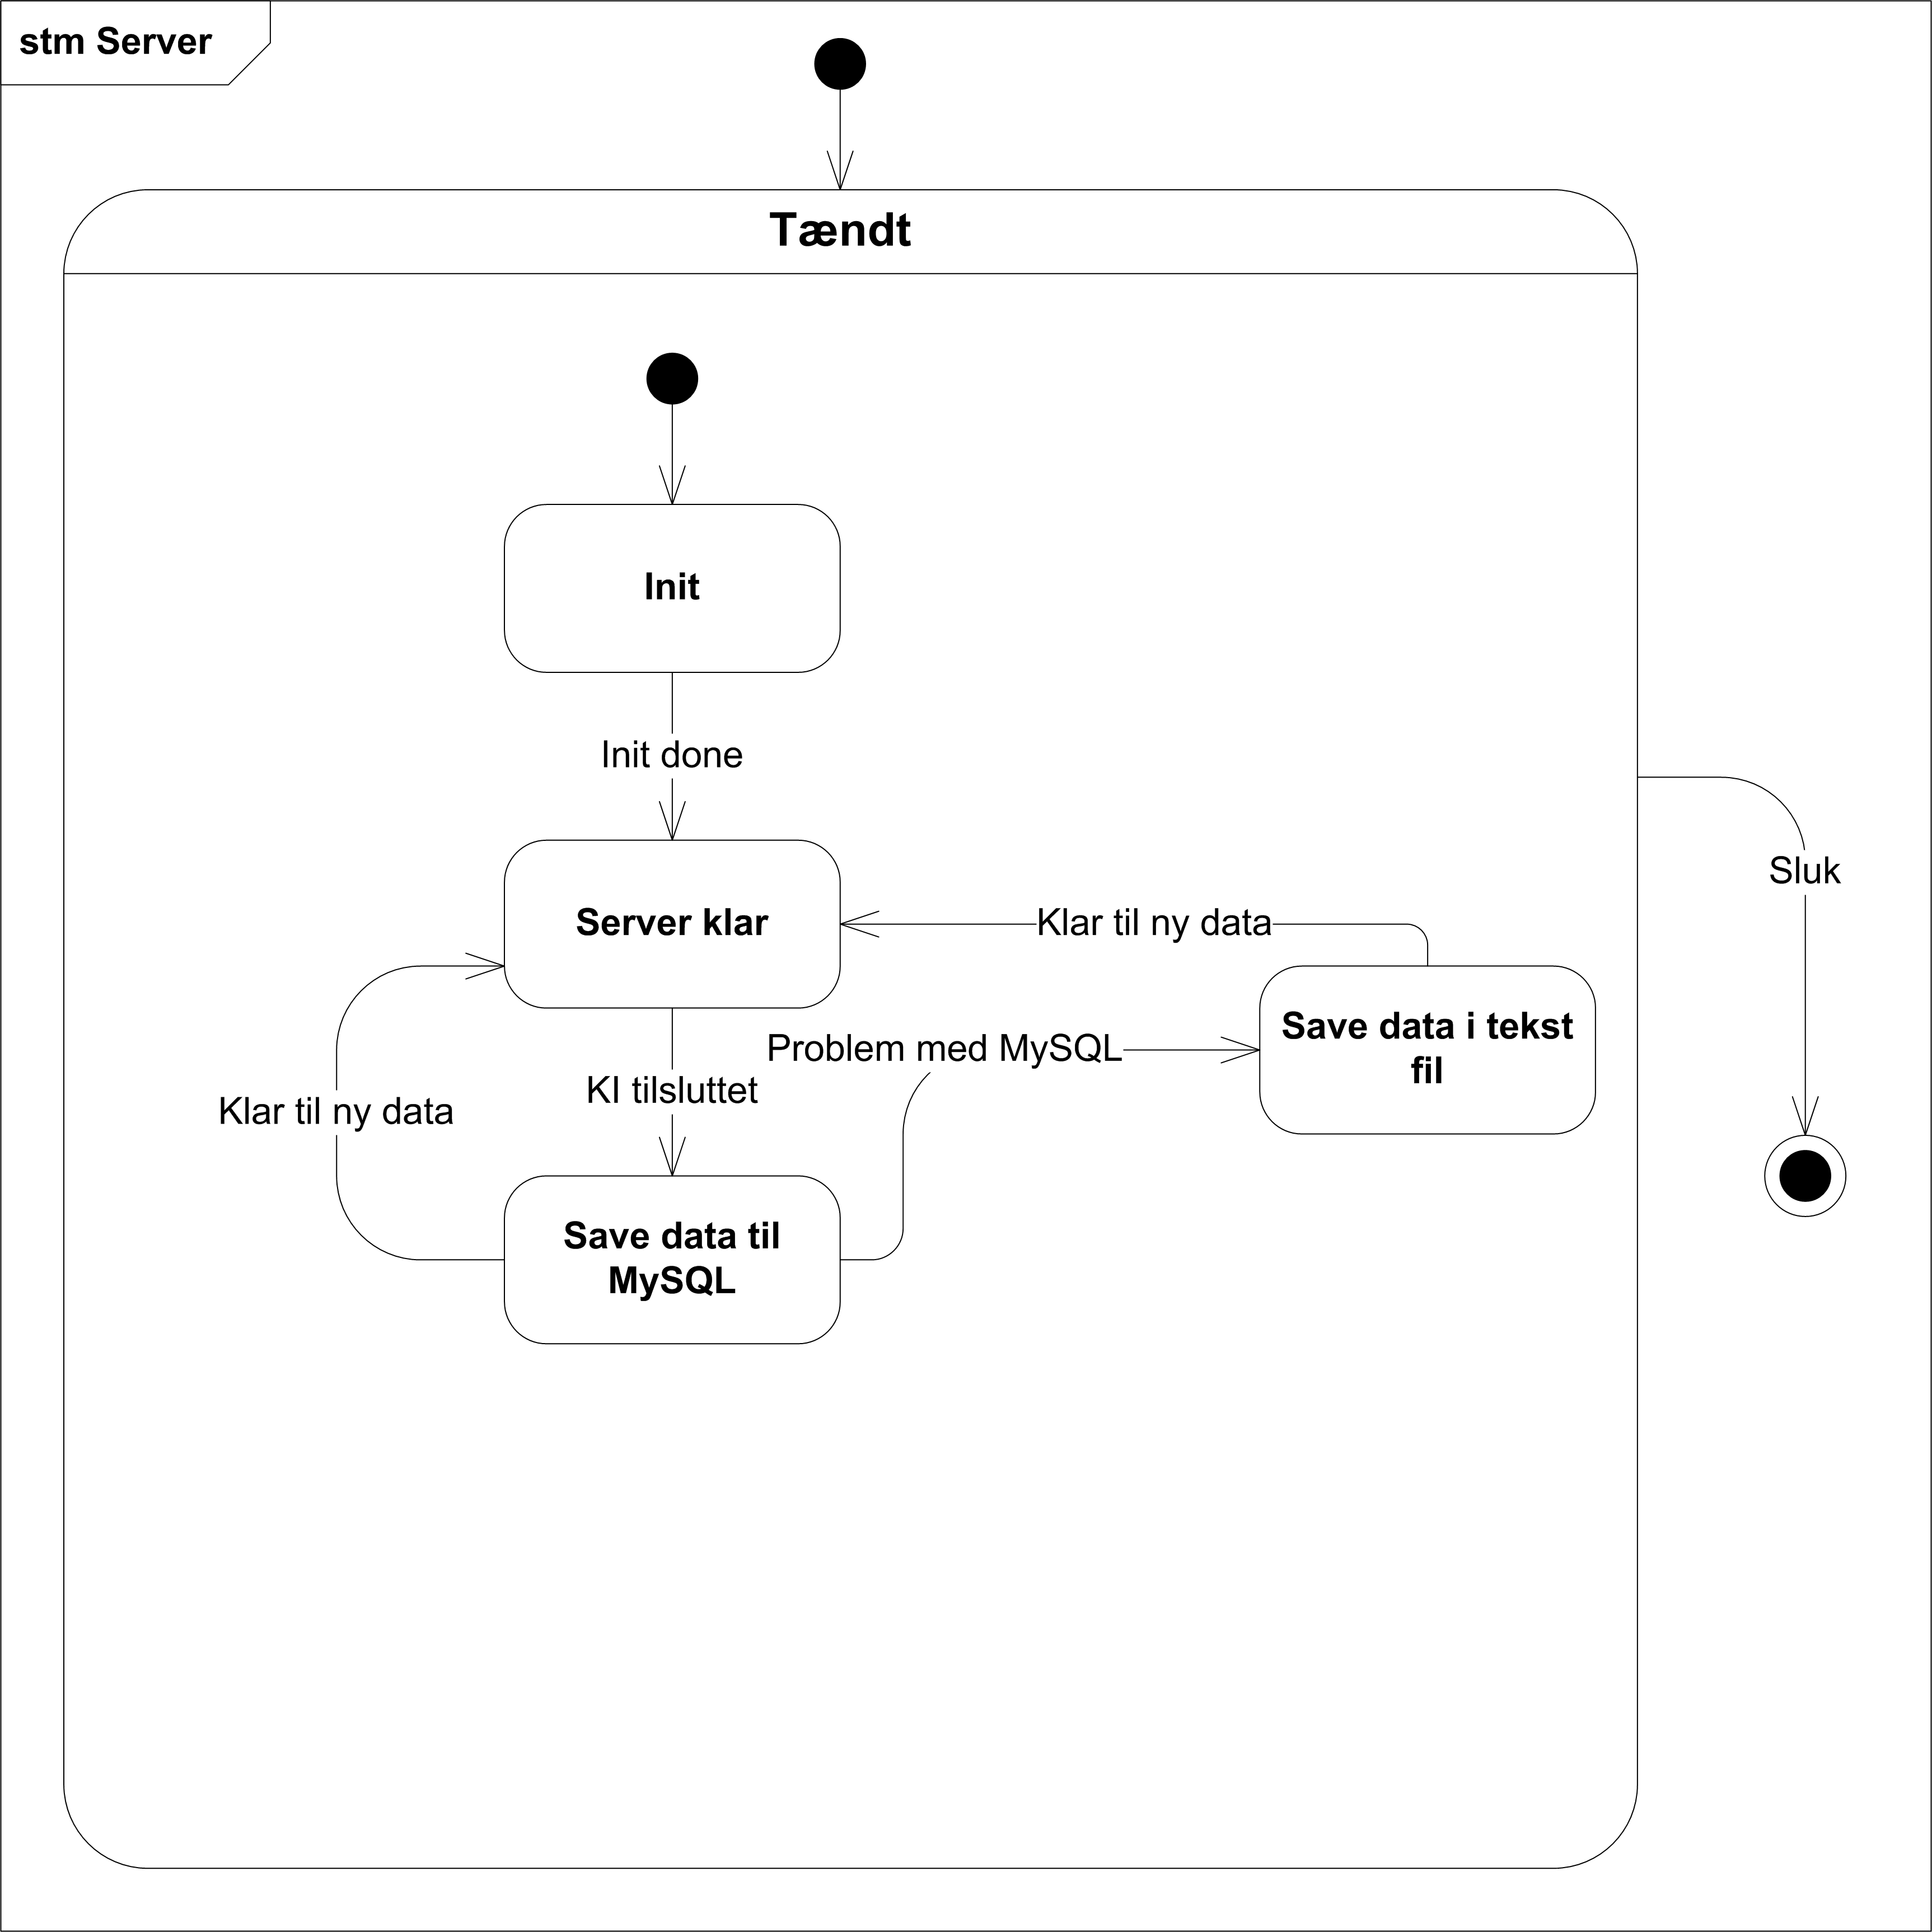
\includegraphics[width=0.6\textwidth]{billeder/Database/stm_server}
	\caption{State machine diagram for serveren}
	\label{fig:stm_server}
\end{figure}

\begin{figure}[H]
	\centering
	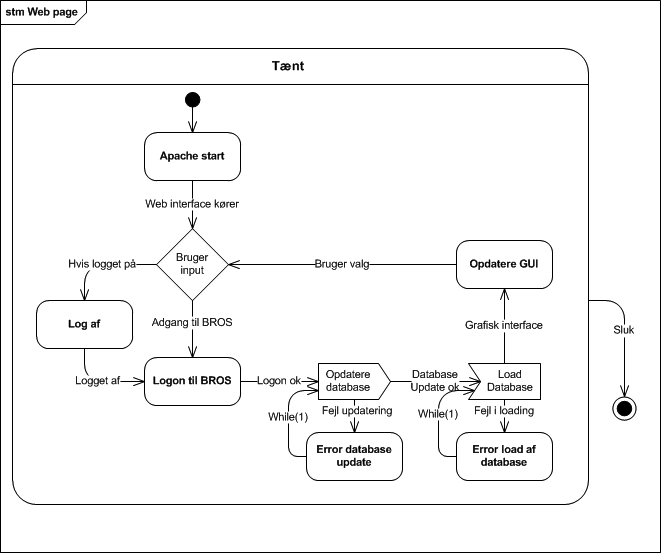
\includegraphics[width=0.6\textwidth]{billeder/Database/stm_web}
	\caption{State machine diagram for serveren}
	\label{fig:stm_web}
\end{figure}

\subsection{Klassediagrammer}
Nedenfor ses klassediagrammerne for databasen. Bemærk databasemodulet er lavet som en serverdel og en webdel\\
Serveredelen er opskrevet som et normalt klassediagram og websiden er opskrevet som et modificeret klassediagram. Dette skyldes at websiden er opbygget som en blanding imellem HTML og php. HTML kan man ikke lave et decideret klassediagram, da der ikke findes funktionskald i dette, men blot includes. Php har derimod funktionskald og er lavet traditionelt. For at lette læsningen af diagrammet har alle blokke i webinterface-klassediagrammet skrevet i toppen om det er HTML eller php.

\begin{figure}[htbp]
	\centering
	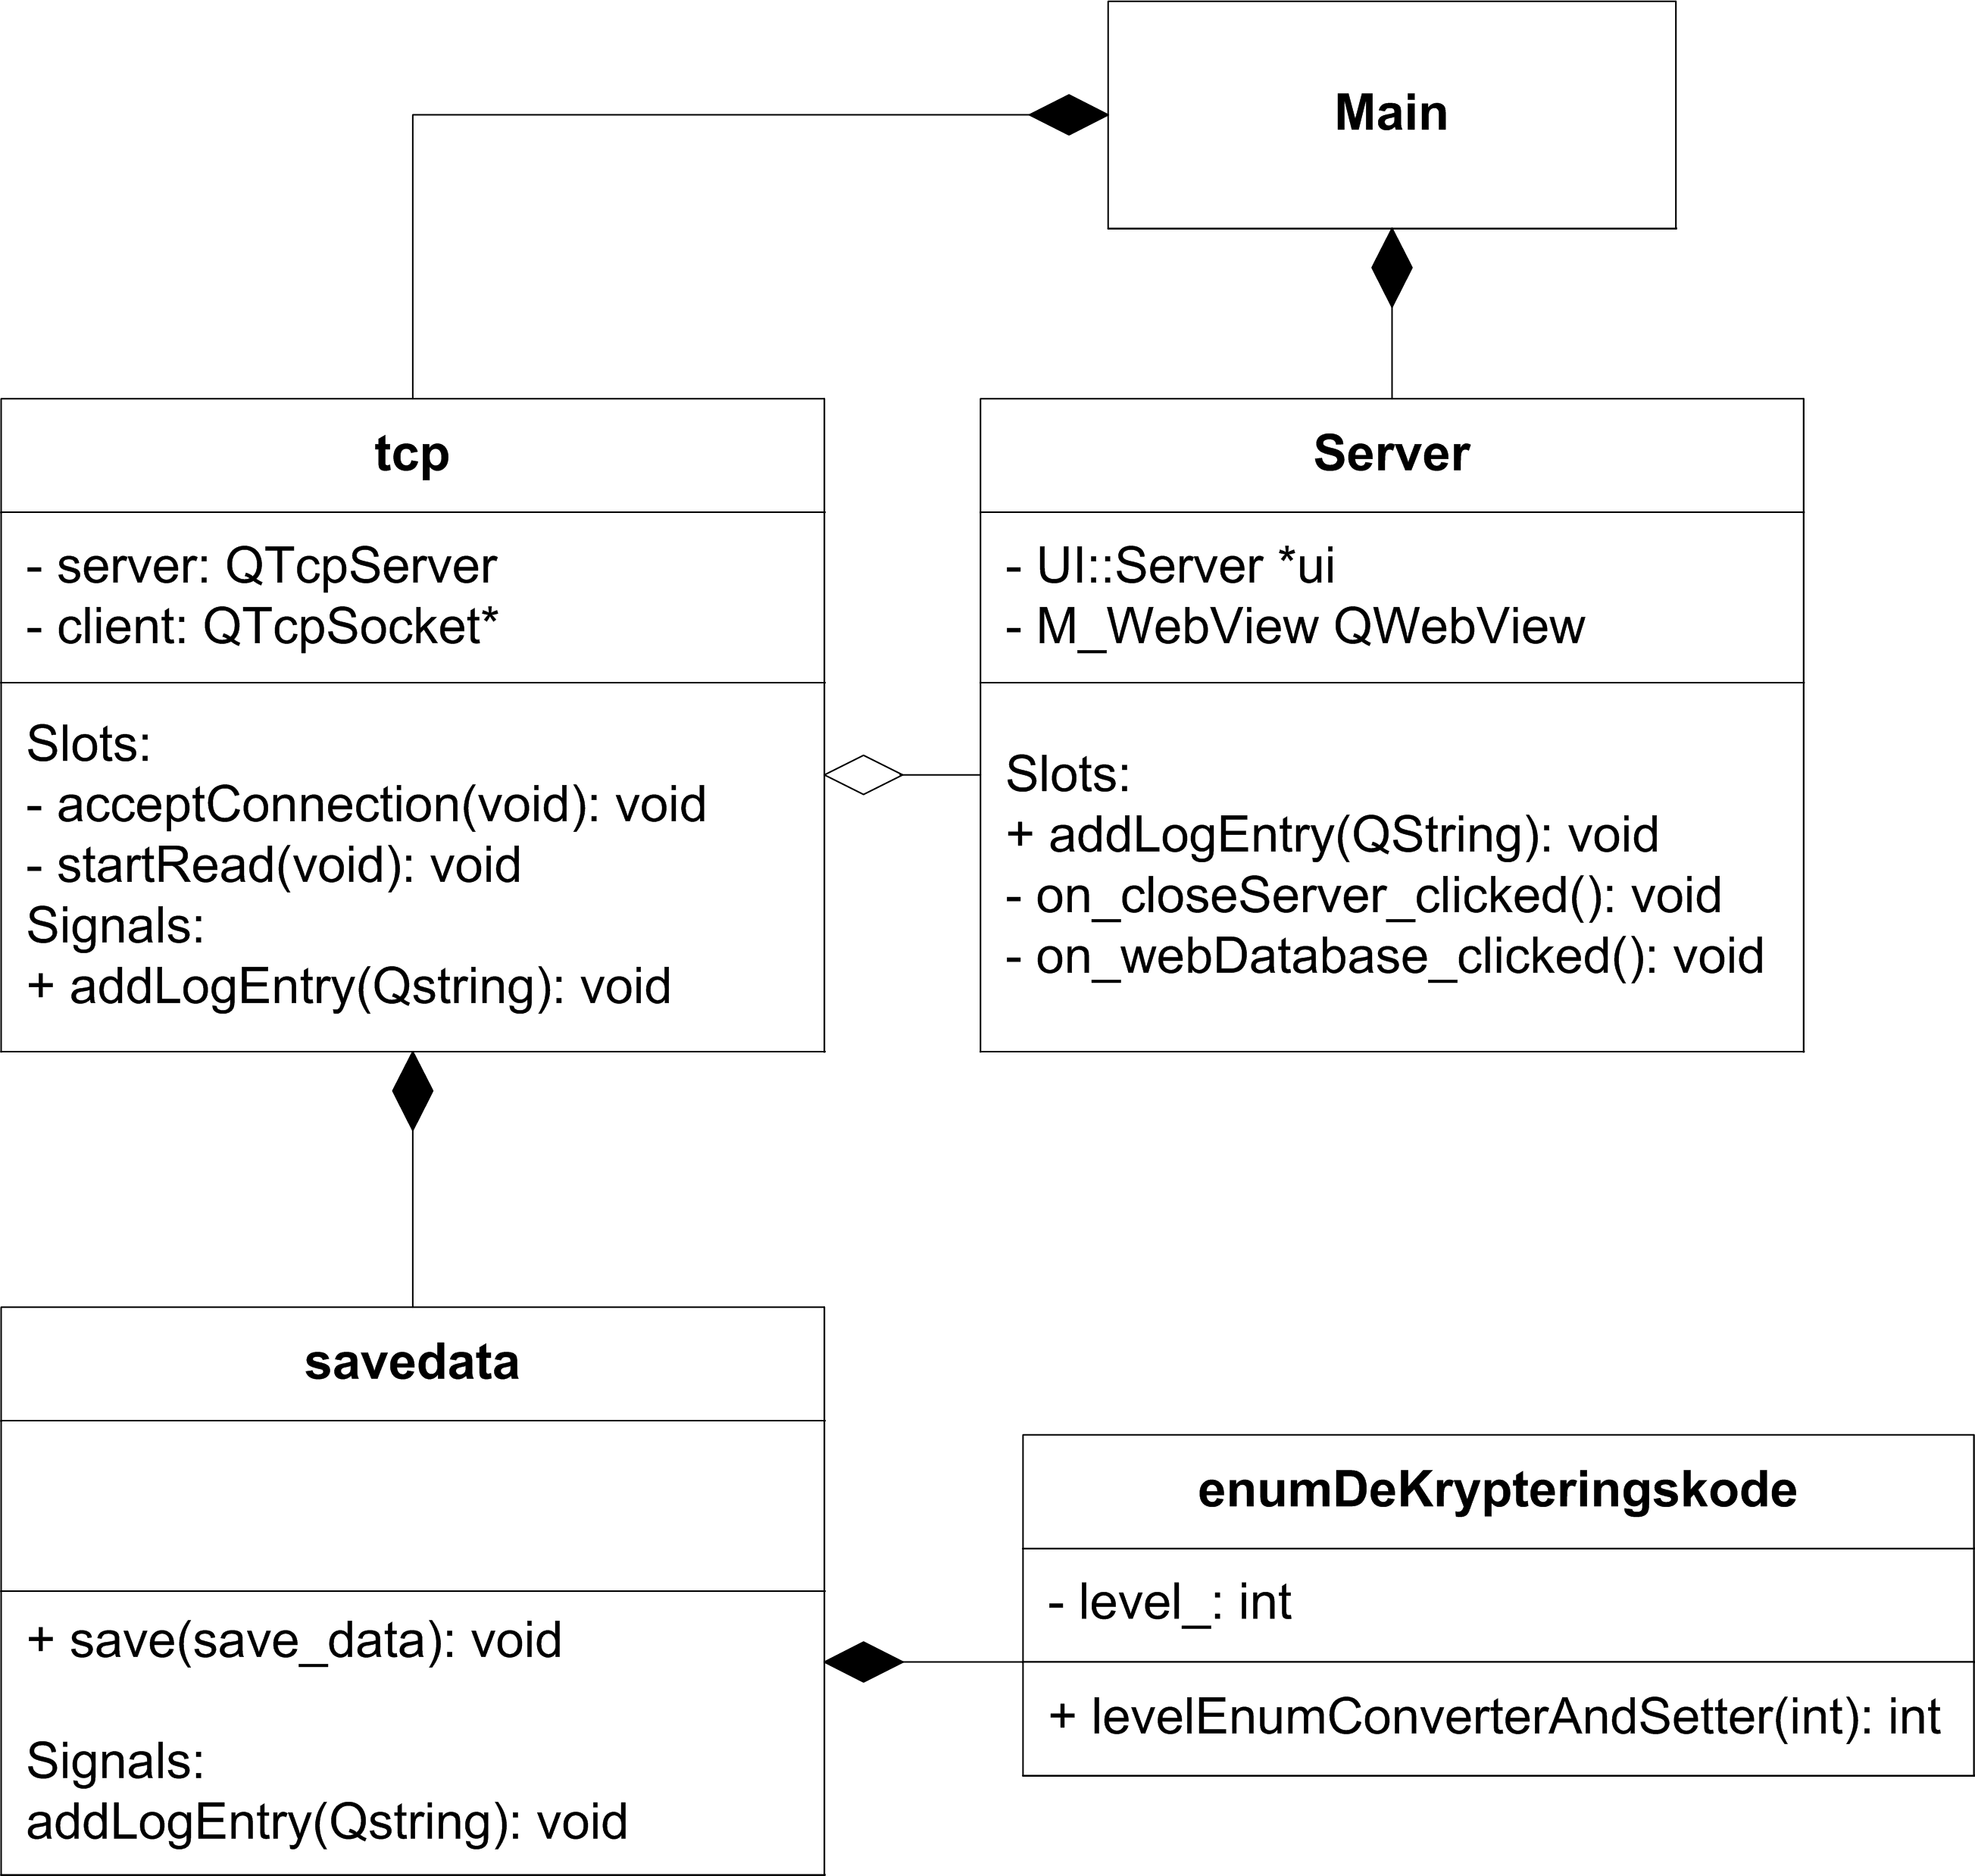
\includegraphics[width=0.4\textwidth]{billeder/Database/serverKlassediagram}
	\caption{Klassedigram for databasens servere}
	\label{fig:serverKlassediagram}
\end{figure}

\begin{table}[H]
\centering
\rowcolors{1}{white}{light-gray}
\begin{tabular}{| p{3cm}  p{12.5cm}|}
\multicolumn{2}{l}{{\Large Serverens klasser}} \\\hline
Server:&Hovedklassen. Denne klasse står for udskrivning til GUI og meddele fejl.\\\hline
tcp:& Står for modtagelse af data fra KI. Denne splitter den modtagede streng og sender den videre til savedata.\\\hline
savedata: & Står for at gemme alle data til en tekstfil.\\\hline
enumDeKrypteringkode:& Står for at dekryptere LEVEL til grader.\\\hline
\end{tabular}
\caption{Serveren klasser}
\label{tabel:server-klasser}
\end{table}

\begin{figure}[H]
	\centering
	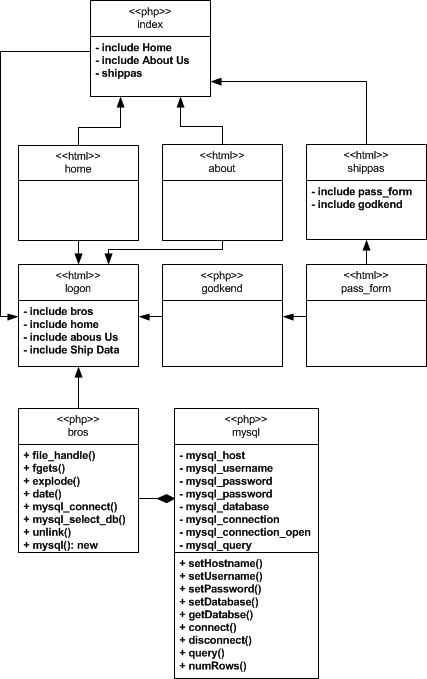
\includegraphics[width=0.5\textwidth]{billeder/Database/web_klasse}
	\caption{Klassedigram for databasens webinterface}
	\label{fig:serverKlassediagram}
\end{figure}

\begin{table}[H]
\centering
\rowcolors{1}{white}{light-gray}
\begin{tabular}{| p{3cm}  p{12.5cm}|}
\multicolumn{2}{l}{{\Large Webinterfacets klasser}} \\\hline
index:& Denne er første side brugeren kommer til. Includer shippas.\\\hline
shippas:& Denne includeres i index og håndtere adgangskoden fra brugeren ved hjælp af pass\_form og godkend.\\\hline
pass\_form: & Indtastningsblokken for adgangskode til databasen.\\\hline
godkend:& Checker om brugeren har tastet korrekt adgangskode, og sender brugeren videre til logon ved korrekt password.\\\hline
logon:& Er hovedsiden i databasen. Denne includere ship og bros. \\\hline
ship:& Denne håndtere de skibe der er tilsluttet BROS database.\\\hline
bros:& Denne gemmer ny data til MySQL databasen. Sletter den filen data var lagret i. Henter og viser alle data i MySQL databasen.\\\hline
mysql:& Tager kontakt til MySQL databasen. opretter forbindelse. Danner en row til håndtering af de data, der skal vises for brugeren.\\\hline
\end{tabular}
\caption{Webinterfacets klasser}
\label{tabel:web-klasser}
\end{table}

\subsection{Funktionsbeskrivelser}
\subsubsection{Server}
Denne header står for at starte serveren og starte GUI for korte informationer til brugeren. Alle informationer om serverstart, connection og datamodtagelse vil blive udskrevet her. 

\begin{table}[H]
\begin{tabular}{l p{12.5cm}}
\multicolumn{2}{l}{\texttt{\textcolor{blue}{Void} addLogEntry( \textcolor{blue}{QString} )}} \\
\hline
Beskrivelse & Står for at udskrive beskeder fra tcp-klassen til GUI \\
Parametre: & Ui::Server *ui;\\
Returværdi:& Ingen\\
\end{tabular}
\end{table}

\begin{table}[H]
\begin{tabular}{l p{12.5cm}}
\multicolumn{2}{l}{\texttt{\textcolor{blue}{Void} on\_closeServer\_clocked( )}} \\
\hline
Beskrivelse: &Denne funktion håndterer luk-knappen. Ved trykknappen, vil brugeren blive bedt om at svare ja eller nej til at lukke serverconnectionen. En knap, der er implementeret som en hjælp, men ikke videre beskrevet \\
Parametre: & Ingen\\
Returværdi: & Ingen\\
\end{tabular}
\end{table}

\begin{table}[H]
\begin{tabular}{l p{12.5cm}}
\multicolumn{2}{l}{\texttt{\textcolor{blue}{Void} on\_webDatabase\_clicked( )}} \\
\hline
Beskrivelse: & Denne funktion står for at håndtere den direkte adgang til den webbaserede database. Ved tryk vil brugeren få åbnet et nyt vindue med databaseadgang \\
Parametre: & QWebView* m\_pWebView\\
Returværdi: & Ingen\\
\end{tabular}
\end{table}

\subsubsection{update}
Denne header indeholder de data, der skal sendes fra tcp-klassen til savedata

\subsubsection{tcp}
Denne header står for at forbindelsen fra KI kan oprettes. Denne opretter en socket og klargør serveren til modtagelse af data. Ved modtagelse af data sørger klassen for opdeling af strengen og flytte dem til variabler for videre behandling

\begin{table}[H]
\begin{tabular}{l p{12.5cm}}
\multicolumn{2}{l}{\texttt{\textcolor{blue}{Void} addLogEntry( \textcolor{blue}{QString} )}} \\
\hline
Beskrivelse: & Står for at udskrive beskeder fra tcp-klassen til GUI \\
Parametre: & Ui::Server *ui;\\
Returværdi:&\\
\end{tabular}
\end{table}

\begin{table}[H]
\begin{tabular}{l p{12.5cm}}
\multicolumn{2}{l}{\texttt{\textcolor{blue}{Void} acceptConnection( \textcolor{blue}{void} )}} \\
\hline
Beskrivelse:&Står for at acceptere forbindelse fra KI og for at tilslutte.\\
Parametre:&QTcpServer server\\
				&QTcpSocket* client\\
Returværdi:&\\
\end{tabular}
\end{table}

\begin{table}[H]
\begin{tabular}{l p{12.5cm}}
\multicolumn{2}{l}{\texttt{\textcolor{blue}{Void} startRead( \textcolor{blue}{void} )}} \\
\hline
Beskrivelse:&Læser data fra socket. Data, som bliver modtaget, som en streng, bliver splittet og lagt ud i de fem variabler ID, STYRBORD, BAGBORD, LEVEL og TIME\\
Parametre:&QTcpSocket* client\\
Returværdi:&\\
\end{tabular}
\end{table}

\subsubsection{enumdekrypteringskode}
Denne header står for at dekryptere LEVEL-niveau til grader fra sm. 

\begin{table}[H]
\begin{tabular}{l p{12.5cm}}
\multicolumn{2}{l}{\texttt{\textcolor{blue}{int} levelEnumConverterAndSetter( \textcolor{blue}{int level} )}} \\
\hline
Beskrivelse & Oversætter LEVEL til grader ud fra protokollen fra uart\\
Parametre: & level\\
Returværdi:& level\\
\end{tabular}
\end{table}



\subsubsection{savedata}
Denne header står for at håndtere lagring af data modtaget fra skibet. Den lagrer dataerne i ship.txt.

\begin{table}[H]
\begin{tabular}{l p{12.5cm}}
\multicolumn{2}{l}{\texttt{\textcolor{blue}{int} save( \textcolor{blue}{save\_data} )}} \\
\hline
Beskrivelse & Står for at gemme data til en tekstfil. \\
Parametre: & Ingen\\
Returværdi:& Ingen\\
\end{tabular}
\end{table}

\subsubsection{Webinterface}
Webinterface står for at fremvise skibsdata grafisk for terminalpersonalet. Desuden står den for at lagre data og loade data fra MySQL-databasen.\\

\subsubsection{bros}

\begin{table}[H]
\begin{tabular}{l p{12.5cm}}
\multicolumn{2}{l}{\texttt{\textcolor{blue}{} file\_handle( \textcolor{blue}{} )}} \\
\hline
Beskrivelse:&Klargør tekstfil til læsning\\
Parametre:& Ingen\\
Returværdi:& Ingen\\
\end{tabular}
\end{table}

\begin{table}[H]
\begin{tabular}{l p{12.5cm}}
\multicolumn{2}{l}{\texttt{\textcolor{blue}{} fgets ( \textcolor{blue}{} )}} \\
\hline
Beskrivelse:&Tager fat i tekststrengen i tekstfilen\\
Parametre:& Ingen\\
Returværdi:& Ingen\\
\end{tabular}
\end{table}

\begin{table}[H]
\begin{tabular}{l p{12.5cm}}
\multicolumn{2}{l}{\texttt{\textcolor{blue}{} explode( \textcolor{blue}{} )}} \\
\hline
Beskrivelse: &Splitter linien op i flere variable\\
Parametre: & Ingen\\
Returværdi: & Ingen\\
\end{tabular}
\end{table}

\begin{table}[H]
\begin{tabular}{l p{12.5cm}}
\multicolumn{2}{l}{\texttt{\textcolor{blue}{} date( \textcolor{blue}{} )}} \\
\hline
Beskrivelse: &Opdaterer dato og tid når der gemmes til MySQL-databasen\\
Parametre: & Ingen\\
Returværdi: & Ingen\\
\end{tabular}
\end{table}

\begin{table}[H]
\begin{tabular}{l p{12.5cm}}
\multicolumn{2}{l}{\texttt{\textcolor{blue}{} mysql\_connect( \textcolor{blue}{} )}} \\
\hline
Beskrivelse: &connecter til MySQL-databasen\\
Parametre: & Ingen\\
Returværdi: & Ingen\\
\end{tabular}
\end{table}

\begin{table}[H]
\begin{tabular}{l p{12.5cm}}
\multicolumn{2}{l}{\texttt{\textcolor{blue}{} mysql\_select\_db( \textcolor{blue}{} )}} \\
\hline
Beskrivelse: & Vælger hvilken database, der skal benyttes i MySQL\\
Parametre: & Ingen\\
Returværdi: & Ingen\\
\end{tabular}
\end{table}

\begin{table}[H]
\begin{tabular}{l p{12.5cm}}
\multicolumn{2}{l}{\texttt{\textcolor{blue}{} unlink( \textcolor{blue}{} )}} \\
\hline
Beskrivelse: & Sletter den tekstfil, som der lige er blevet læst fra\\
Parametre: & Ingen\\
Returværdi: & Ingen\\
\end{tabular}
\end{table}

\begin{table}[H]
\begin{tabular}{l p{12.5cm}}
\multicolumn{2}{l}{\texttt{\textcolor{blue}{new} mysql( \textcolor{blue}{} )}} \\
\hline
Beskrivelse: & Opretter ny databaseforbindelse\\
Parametre: & Ingen\\
Returværdi: & Ingen\\
\end{tabular}
\end{table}

\subsubsection{mysql}
\begin{table}[H]
\begin{tabular}{l p{12.5cm}}
\multicolumn{2}{l}{\texttt{\textcolor{blue}{} setHostName( \textcolor{blue}{} )}} \\
\hline
Beskrivelse: & Sætter servernavn/serverip\\
Parametre: & Ingen\\
Returværdi: & Ingen\\
\end{tabular}
\end{table}

\begin{table}[H]
\begin{tabular}{l p{12.5cm}}
\multicolumn{2}{l}{\texttt{\textcolor{blue}{} setUserName( \textcolor{blue}{} )}} \\
\hline
Beskrivelse: & Skriver brugernavn til databasen\\
Parametre: & Ingen\\
Returværdi: & Ingen\\
\end{tabular}
\end{table}

\begin{table}[H]
\begin{tabular}{l p{12.5cm}}
\multicolumn{2}{l}{\texttt{\textcolor{blue}{} setPassword( \textcolor{blue}{} )}} \\
\hline
Beskrivelse:&Skriver password til databasen\\
Parametre: & Ingen\\
Returværdi: & Ingen\\
\end{tabular}
\end{table}

\begin{table}[H]
\begin{tabular}{l p{12.5cm}}
\multicolumn{2}{l}{\texttt{\textcolor{blue}{} setDatabase( \textcolor{blue}{} )}} \\
\hline
Beskrivelse: & Fortæller MySQL hvilken database, der skal benyttes\\
Parametre: & Ingen\\
Returværdi: & Ingen\\
\end{tabular}
\end{table}

\begin{table}[H]
\begin{tabular}{l p{12.5cm}}
\multicolumn{2}{l}{\texttt{\textcolor{blue}{} getDatabase( \textcolor{blue}{} )}} \\
\hline
Beskrivelse: & Tager fat i databasen\\
Parametre: & Ingen\\
Returværdi: & Ingen\\
\end{tabular}
\end{table}

\begin{table}[H]
\begin{tabular}{l p{12.5cm}}
\multicolumn{2}{l}{\texttt{\textcolor{blue}{} connect( \textcolor{blue}{} )}} \\
\hline
Beskrivelse: & Står for at samle localhost, username, password, database og connecte til databasen\\
Parametre: & Ingen\\
Returværdi: & Ingen\\
\end{tabular}
\end{table}

\begin{table}[H]
\begin{tabular}{l p{12.5cm}}
\multicolumn{2}{l}{\texttt{\textcolor{blue}{} disconnect( \textcolor{blue}{} )}} \\
\hline
Beskrivelse: & Lukker databaseforbindelsen\\
Parametre: & Ingen\\
Returværdi: & Ingen\\
\end{tabular}
\end{table}

\begin{table}[H]
\begin{tabular}{l p{12.5cm}}
\multicolumn{2}{l}{\texttt{\textcolor{blue}{} query( \textcolor{blue}{} )}} \\
\hline
Beskrivelse: & Opretter databasekø og skriver data til skærm\\
Parametre: & Ingen\\
Returværdi: & Ingen\\
\end{tabular}
\end{table}

\begin{table}[H]
\begin{tabular}{l p{12.5cm}}
\multicolumn{2}{l}{\texttt{\textcolor{blue}{} numRows( \textcolor{blue}{} )}} \\
\hline
Beskrivelse: & Checker hvor mange rækker der findes i databasen. Bruges desuden til at udskrive om databasen er tom.\\
Parametre: & Ingen\\
Returværdi: & Ingen\\
\end{tabular}
\end{table}

\subsection{Tilpasning}
Der er mulighed for at opsætte serverdelen sådan at denne lagrer direkte i MySQL-databasen hvis man har et ønske om at mindske ansvaret for websiden. For at gøre dette, kan man i tcp-klassens funktion startRead(void) erstatte funktionskaldet til klassen savedata() med funktionen save(tmp) og i stedet benytte klassen SQL med funktionskaldet saveSQL(tmp). funktionen saveSQL(tmp) har save(tmp) som, i tilfælde af at der opstår fejl med at gemme data til databasen, vil sikre at data bliver lagret i en backupfil, som så kan håndteres af websiden.

\subsection{Apache}
Apache HTTP-Server er en webserver fra Apache Software Foundation. Apache er en ofte benyttet webserver og er en open source-serverprogram. Serveren installeres på en computer og kan herefter benytte ved at benyttes den lokale ip-adresse 127.0.0.1 eller localhost. 'hvis computeren med Apache-serveren er placeret i et større netværk og skal benyttes fra andre computere, kan denne tilgås fra disse ved at indtaste computerens oprindelige ip-adresse på netværket. Dette giver også mulighed for at benytte serveren fra internettet ved at koble den op via DNS. Hvis dette gøres, skal man specielt være opmærksom på at lukke portnumrerne 20 og 21, da disse ofte er portene, som bliver hacket. Desuden bør man ligge adgangskode på serveren for uautoriseret brug. I BROS er Apache-serveren placeret i et internt netværk og derfor er det ikke nødvendigt at lukke portene eller benytte sig af adgangskodetilladelse for at arbejde til serveren.
Generelt står apache-serverene for ca 60\% af alle webserere i verden.
fxnote{kilde: IKN bog og wikipedia} 

\subsection{mySQL}
MySQL er en flertrådet SQL-databaseserver, som understøtter mange samtidige brugere. SQL(Structured Query Language) er det mest populære databasesprog i dag. MySQL'er et klient-/serverprogram, der består af en server (mysqld) og mange forskellige klientprogrammer.\\
MySQL er bygget op omkring forskellige databaser på en server, ofte har hver enkelt bruger en speciel adgang til en databse med en overordnet root-bruger, der har adgang til alle databaser.\\
MySQL er en relationel database, hvori man kan oprette flere tabeller til at håndtere flere ting. I BROSdatabasen benyttes der en database med navnet bros. I denne database kan der oprettes tabeller til de skibe, der skal kunne gemmes data for. C++ og php er i stand til at se på om en tabel er oprettet. Hvis den ikke er det, kan sprogene selv oprette disse(dette er ikke indkodet, da vi kun arbejder med et skib). \\
For at tilgå mySQL kan man benytte sig af terminalen \footnote{beskrevet i apendix} eller grafisk brugergrænseflade som f.eks. phpMyAdmin (benyttet under udviklingen).
MySQL kan benytte flere forskellige datatyper, som vil blive beskrevet i apandix for MySQL. 






